\documentclass[aspectratio=43,t]{beamer}
%\documentclass[aspectratio=43,t,handout]{beamer}

\usepackage[ansinew]{inputenc}
\usepackage[T1]{fontenc}
%English version FAU Logo
\usepackage[english]{babel}
%German version FAU Logo
%\usepackage[ngerman]{babel}
\usepackage{amsmath,amssymb}
\usepackage{graphicx}
\usepackage{wrapfig}
\usepackage{listings}
\usepackage[backend=biber,sorting=none,doi=true,style=ieee]{biblatex}

% Themes:
%  - fau:          FAU theme
%  - fau-med:      MedFak FAU theme
%  - fau-nat:      NatFak FAU theme
%  - fau-phil:     PhilFak FAU theme
%  - fau-rw:       RWFak FAU theme
%  - fau-rw-jura:  RWFak FB Jura FAU theme
%  - fau-rw-wiso:  RWFak FB WISO FAU theme
%  - fau-tf:       TechFak FAU theme
%
% Options:
%  - image:        Cover image on title page
%  - plain:        Plain title page
%  - longtitle:    Title page layout for long title
\usetheme[longtitle]{fau-tf}

% Enable semi-transparent animation preview
\setbeamercovered{transparent}


\lstset{%
  language=C++,
  tabsize=2,
  basicstyle=\tt\scriptsize,
  keywordstyle=\color{blue},
  commentstyle=\color{green!50!black},
  stringstyle=\color{red},
  numbers=left,
  numbersep=0.5em,
  numberstyle=\tt\tiny
}


\defbibheading{bibliography}{}
\addbibresource[label=primary]{references.bib}
\nocite{*}


% Title, authors, and date
\title[Ray Tracing Simulation of optically pumped Laser Crystals]{Ray Tracing Simulation of optically pumped Laser Crystals}
\subtitle{Masters Project}
\author[Matthias Koenig]{Matthias Koenig}
% English version
\institute[FAU LSS]{Chair for Computer Science 10, System Simulation, Friedrich-Alexander University of Erlangen-Nuremberg}
% German version
%\institute[Lehrstuhl f\"ur XYZ]{Lehrstuhl f\"ur XYZ, Friedrich-Alexander-Universit\"at Erlangen-N\"urnberg}
\date{\today}
% Set additional logo (overwrites FAU seal)
%\logo{\includegraphics[width=.15\textwidth]{themefau/art/xxx/xxx.pdf}}


\begin{document}
  % Title
  \maketitle

  { % Motivation
    \setbeamertemplate{footline}{}
    \begin{frame}[fragile]{Motivation}
		
		\begin{figure}
		\centering
		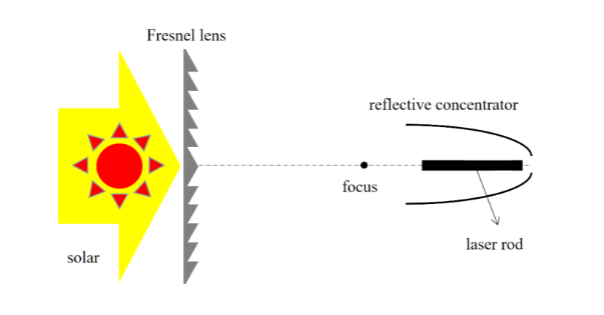
\includegraphics[width=0.65\textwidth]{images/setup.png}
		\end{figure}

    \begin{block}{Problems to solve:}
      \begin{enumerate}
				\item<2-> Build a framework for physically accurate raytracing
        \item<3-> Calculate absorbed power
        \item<4-> Optimize mirror shape
      \end{enumerate}
    \end{block}
		
		In the Masters Project a 2D proof of concept was developed.

    \end{frame}
  }

  { % Outline
    \setbeamertemplate{footline}{}
    \begin{frame}[noframenumbering]{Outline}
      \tableofcontents
    \end{frame}
  }

	\section{Ray Tracing Basics}
    \begin{frame}[fragile]{Parametrization}
		
		All points along a ray are described as follows:

		\begin{equation*}
			\boldsymbol{r}(t) = \boldsymbol{o} + t \cdot \boldsymbol{d}
		\end{equation*}

		Testing intersections against primitives involves solving for the parameter $t$.\\
		\textbf{Example:} Axis aligned box intersection\\
		
		\begin{figure}
		\centering
		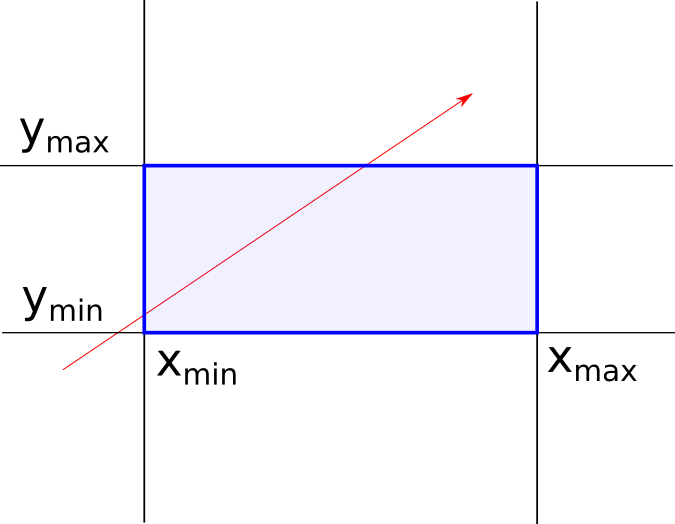
\includegraphics[width=0.5\textwidth]{images/aabb.png}
		\end{figure}
    \end{frame}

    \begin{frame}[fragile]{Parametrization contd.}
			\textbf{Solution:} \\
			\bigskip
			
		\begin{lstlisting}[language=C++]
  	float tx1 = (xmin - ray.origin.x) / ray.direction.x;
  	float tx2 = (xmax - ray.origin.x) / ray.direction.x;

  	float tmin = min(tx1, tx2);
  	float tmax = max(tx1, tx2);

  	float ty1 = (ymin - ray.origin.y) / ray.direction.y;
  	float ty2 = (ymax - ray.origin.y) / ray.direction.y;

  	tmin = max(tmin, glm::min(ty1, ty2));
  	tmax = min(tmax, glm::max(ty1, ty2));
		\end{lstlisting}
		\bigskip
		Other primitives in 2D can be lines, cricles, etc.\\
		Or in 3D triangles, quads, spheres, etc.\\
		\bigskip
		All objects in a scene need to be built with a collection of such primitives.
    \end{frame}

	\section{Scene Tracing}

    \begin{frame}[fragile]{Scene Tracing}
			If a ray hits an object new rays are genertated according to its type
			of surface (reflection, refraction).\\
			\bigskip
			These new rays are traced again through the scene.\\
			\bigskip
			$\implies$ Recurse until a desired "depth".\\
			\bigskip
			An object is intersected if one of its primitives is hit.\\
			\bigskip
			$\implies$ Need to check each primitive of every object in the scene.\\
			\bigskip
			Runtime of a scene tracing step with $N$ objects with $M$ primitives each:

			\begin{equation*}
				O(N * M)
			\end{equation*}
    \end{frame}

    \begin{frame}[fragile]{Hierarchical Bounding Volumes}
			Performance optimization:\\
			\bigskip
      \begin{enumerate}
				\item<2-> Preprocessing: Attach a bounding box around each object and 
					recursively subdivide.
				\item<3-> Tracing: Check if ray hits bounding box. If yes recursively check its
					subdivisions.
      \end{enumerate}
			\bigskip
			Runtime of a scene tracing step with $N$ objects with $M$ primitives each
			and 5 recursive subdivisions:

			\begin{equation*}
				O(N * (5*4 + M/4^5)) = O(N * M/1024)
			\end{equation*}
    \end{frame}

    \begin{frame}[fragile]{Mirror}
			Mirror consists of 2D line segments arranged by a 1D shape function (parabolic for testing
			purposes).

			\begin{figure}
			\centering
			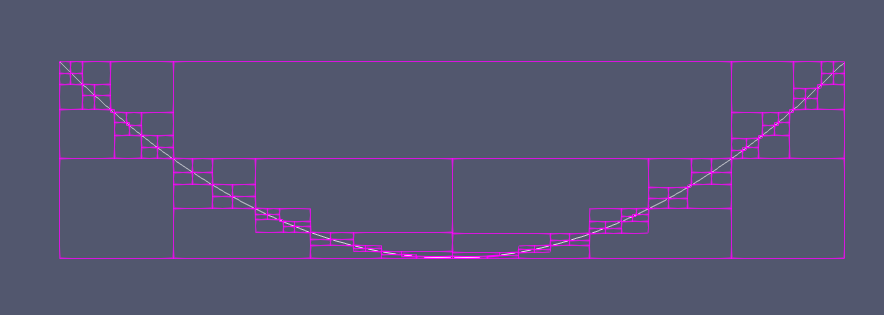
\includegraphics[width=0.8\textwidth]{images/mirror.png}
			\end{figure}

    \end{frame}

    \begin{frame}[fragile]{Crystal}
			The laser crystal is a 2D Box with an internal grid structure and grid tracing algorithm.\\
			Rays need to be traced through cells \textbf{in order}\footnote{A Fast Voxel Traversal Algorithm for Ray Tracing, John Amanatides, Andrew Woo, University of Toronto} because 
			of the absorbed energy calculation.\\

			\begin{figure}
			\centering
			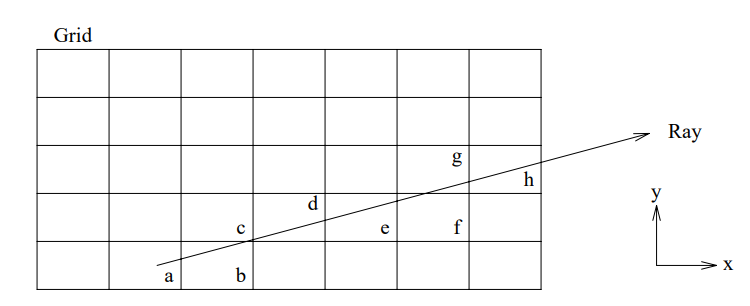
\includegraphics[width=0.8\textwidth]{images/grid.png}
			\end{figure}


    \end{frame}

	\section{Sampling Techniques}

    \begin{frame}[fragile]{Generating Rays and Random Sampling}
		The goal is to randomly generate a cone of rays originating in the focus
		of the fresnel lense.\\
		\bigskip
		$\implies$ Uniformly sample the opening angle around a direction vector.

		\begin{figure}
		\centering
		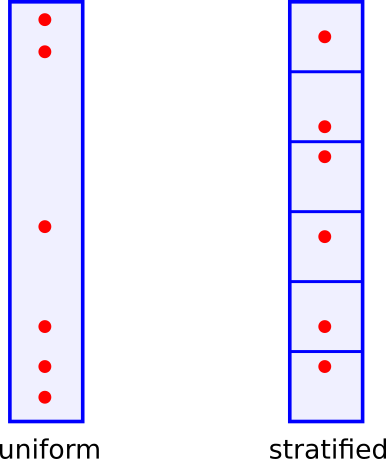
\includegraphics[width=0.3\textwidth]{images/stratified.png}
		\end{figure}

		\bigskip
		$\implies$ Not ideal in this case (big gaps between rays)\\
		$\implies$ Better: Stratified Uniform Sampling
		\end{frame}

		\begin{frame}[fragile]{Inversion Method}
		In reality sunlight consists of unpolarized light with a specific frequency spectrum.\\
		Thus the rays need to carry information about their power, frequency and polarity.\\
		\bigskip
		$\implies$ Need mechanism to generate random samples $x$ according to 
			a given distribution density function $p(x)$ (gauss, poisson, sun spectrum, etc.)\\
		\bigskip
			\textbf{Inversion Method:}\\
      \begin{enumerate}
				\item<2-> Integrate(sum up) the distribution $p(x)$ in uniform steps $x$ and save
					the value for each step resulting in $P(x)$.
				\item<3-> Uniformly sample $\xi \in [0,1]$ and figure out in which interval it lies.
        \item<4-> Interpolate linearly within the interval and return resulting $x$ value.
      \end{enumerate}

		\bigskip
		\bigskip
		Frequencies and polarisations of rays are not implemented as of yet.
    \end{frame}

		\begin{frame}[fragile]{Inversion Method contd.}
		\begin{figure}
		\centering
		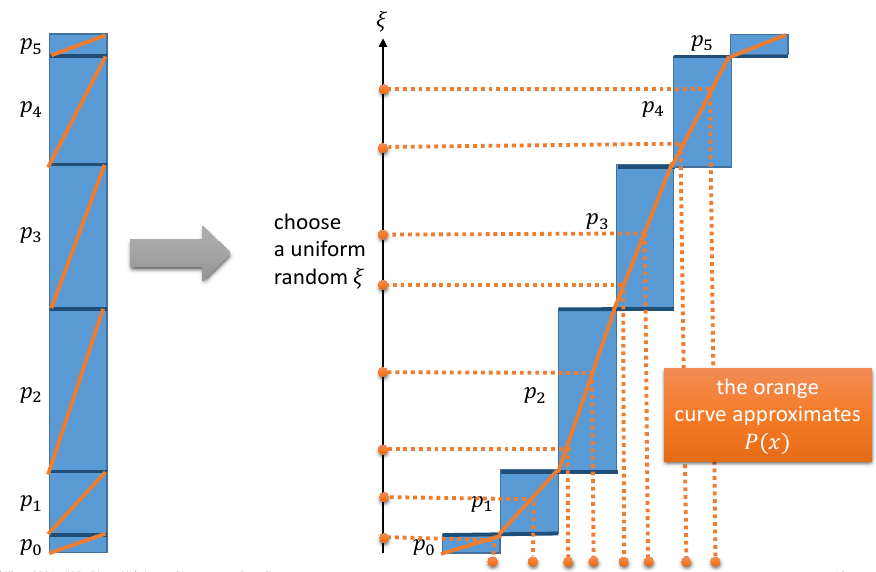
\includegraphics[width=0.8\textwidth]{images/inversion.png}
		\end{figure}
    \end{frame}

	\section{Reflection and Refraction}

		\begin{frame}[fragile]{Reflection}
		A ray is reflected by creating a new ray with the origin at the intersection
		point and the direction determined by the incident angle.

		\bigskip

		\begin{equation*}
			\theta_1 = \theta_2
		\end{equation*}

		\bigskip

		where $\theta_1$ is the incident angle and $\theta_2$ is the reflection angle.
    \end{frame}

		\begin{frame}[fragile]{Refraction}
		Refraction is modelled accurately by Snells' law:

		\begin{equation*}
			n_1 \sin (\theta_1) = n_2 \sin (\theta_2)
		\end{equation*}

		where $n_1$, $n_2$ are the indices of refraction.

		\begin{figure}
		\centering
		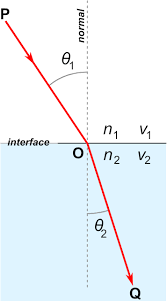
\includegraphics[width=0.25\textwidth]{images/snell.png}
		\end{figure}

    \end{frame}

		\begin{frame}[fragile]{Fresnel Laws}
		The transmitted and reflected power can be calculated with the transmission- and 
			reflection rates given by Fresnel's laws.\\
			These are dependent on the orientation of the polarization of the incident
			ray (perpendicular or parallel) to the surface:\\

		\begin{equation*}
			R_{\perp} = \frac{\sin^2(\theta_1 - \theta_2)}{\sin^2(\theta_1 + \theta_2)}
		\end{equation*}

		\begin{equation*}
			R_{\parallel} = \frac{\tan^2(\theta_1 - \theta_2)}{\tan^2(\theta_1 + \theta_2)}
		\end{equation*}

		\begin{equation*}
			T_{\perp} = 1 - R_{\perp}
		\end{equation*}

		\begin{equation*}
			T_{\parallel} = 1 - R_{\parallel}
		\end{equation*}
    \end{frame}

		\begin{frame}[fragile]{Fresnel Laws contd.}
		For now unpolarized light is assumed and only one refraction takes place so the total
		rates are:

		\begin{equation*}
			R_{total} = \frac{R_{\perp} + R_{\parallel}}{2}
		\end{equation*}

		\begin{equation*}
			T_{total} = \frac{T_{\perp} + T_{\parallel}}{2}
		\end{equation*}

		This will be changed in the future since in reality absorption in the crystal also
		depends on polarization.
    \end{frame}

	\section{Calculating Absorbed Power}
		\begin{frame}[fragile]{Calculating Absorbed Power}
			The remaining power of a ray passing through the crystal is calculated by:

			\begin{equation*}
				I_{out} = I_{in} \cdot e^{-\alpha d}
			\end{equation*}

			where $\alpha$ is the absorption coefficient $d$ is the distance travelled
			through a cell.\\
			Thus the absorbed power is:

			\begin{equation*}
				I_{abs} = I_{in} - I_{out}
			\end{equation*}

			In reality the $\alpha$ is frequency dependent but this is not implemented yet.
    \end{frame}
	\section{Outlook for Masters Thesis}

		\begin{frame}[fragile]{Outlook}
    \begin{block}{Todo:}
      \begin{enumerate}
				\item<2-> Implement custom distribution sampling
        \item<3-> Use frequency and polarity in raytracing/absorption
				\item<4-> Make step to 3D or correct 2D values for 3D usage (transversal rays cannot
					be modelled).
        \item<5-> Optimize mirror shape using freeform shape functions
        \item<6-> Model the Fresnel lense and divergent sunlight
      \end{enumerate}
    \end{block}
    \end{frame}

  { % Questions?
    \setbeamertemplate{footline}{}
    \begin{frame}[c,noframenumbering]
      \begin{center}
        Thanks for listening.\\
        {\bf Any questions/suggestions?}
      \end{center}
    \end{frame}

    % References
    \section*{References}
    \begin{frame}[allowframebreaks,noframenumbering]{References}
      \printbibliography
    \end{frame}
  }
	\end{document}

